\documentclass[onesided]{article}\usepackage[]{graphicx}\usepackage[]{color}
% maxwidth is the original width if it is less than linewidth
% otherwise use linewidth (to make sure the graphics do not exceed the margin)
\makeatletter
\def\maxwidth{ %
  \ifdim\Gin@nat@width>\linewidth
    \linewidth
  \else
    \Gin@nat@width
  \fi
}
\makeatother

\definecolor{fgcolor}{rgb}{0.345, 0.345, 0.345}
\newcommand{\hlnum}[1]{\textcolor[rgb]{0.686,0.059,0.569}{#1}}%
\newcommand{\hlstr}[1]{\textcolor[rgb]{0.192,0.494,0.8}{#1}}%
\newcommand{\hlcom}[1]{\textcolor[rgb]{0.678,0.584,0.686}{\textit{#1}}}%
\newcommand{\hlopt}[1]{\textcolor[rgb]{0,0,0}{#1}}%
\newcommand{\hlstd}[1]{\textcolor[rgb]{0.345,0.345,0.345}{#1}}%
\newcommand{\hlkwa}[1]{\textcolor[rgb]{0.161,0.373,0.58}{\textbf{#1}}}%
\newcommand{\hlkwb}[1]{\textcolor[rgb]{0.69,0.353,0.396}{#1}}%
\newcommand{\hlkwc}[1]{\textcolor[rgb]{0.333,0.667,0.333}{#1}}%
\newcommand{\hlkwd}[1]{\textcolor[rgb]{0.737,0.353,0.396}{\textbf{#1}}}%
\let\hlipl\hlkwb

\usepackage{framed}
\makeatletter
\newenvironment{kframe}{%
 \def\at@end@of@kframe{}%
 \ifinner\ifhmode%
  \def\at@end@of@kframe{\end{minipage}}%
  \begin{minipage}{\columnwidth}%
 \fi\fi%
 \def\FrameCommand##1{\hskip\@totalleftmargin \hskip-\fboxsep
 \colorbox{shadecolor}{##1}\hskip-\fboxsep
     % There is no \\@totalrightmargin, so:
     \hskip-\linewidth \hskip-\@totalleftmargin \hskip\columnwidth}%
 \MakeFramed {\advance\hsize-\width
   \@totalleftmargin\z@ \linewidth\hsize
   \@setminipage}}%
 {\par\unskip\endMakeFramed%
 \at@end@of@kframe}
\makeatother

\definecolor{shadecolor}{rgb}{.97, .97, .97}
\definecolor{messagecolor}{rgb}{0, 0, 0}
\definecolor{warningcolor}{rgb}{1, 0, 1}
\definecolor{errorcolor}{rgb}{1, 0, 0}
\newenvironment{knitrout}{}{} % an empty environment to be redefined in TeX

\usepackage{alltt}
\usepackage[T1]{fontenc}
\linespread{1.5} % Line spacing - Palatino needs more space between lines
\usepackage{microtype} % Slightly tweak font spacing for aesthetics

\usepackage[hmarginratio=1:1,columnsep=20pt]{geometry} % Document margins
%\usepackage{multicol} % Used for the two-column layout of the document
\usepackage[hang, small,labelfont=bf,up,textfont=it,up]{caption} % Custom captions under/above floats in tables or figures
\usepackage{booktabs} % Horizontal rules in tables
\usepackage{float} % Required for tables and figures in the multi-column environment - they need to be placed in specific locations with the [H] (e.g. \begin{table}[H])

\usepackage{lettrine} % The lettrine is the first enlarged letter at the beginning of the text
\usepackage{paralist} % Used for the compactitem environment which makes bullet points with less space between them

% to ignore texts: good for thank messages and paper submissions.
      % \fbox{\phantom{This text will be invisible too, but a box will be printed arround it.}}

\usepackage{abstract} % Allows abstract customization
\renewcommand{\abstractnamefont}{\normalfont\bfseries} % Set the "Abstract" text to bold
%\renewcommand{\abstracttextfont}{\normalfont\small\itshape} % Set the abstract itself to small italic text

\usepackage[]{titlesec} % Allows customization of titles
\renewcommand\thesection{\Roman{section}} % Roman numerals for the sections
\renewcommand\thesubsection{\Roman{subsection}} % Roman numerals for subsections
\titleformat{\section}[block]{\large\scshape\centering}{\thesection.}{1em}{} % Change the look of the section titles
\titleformat{\subsection}[block]{\large}{\thesubsection.}{1em}{} % Change the look of the section titles

\usepackage{fancybox, fancyvrb, calc}
\usepackage[svgnames]{xcolor}
\usepackage{epigraph}
\usepackage{longtable}
\usepackage{pdflscape}
\usepackage{graphics}
\usepackage{pbox} % \pbox{20cm}{This is the first \\ cell}
\usepackage{amsfonts}
\usepackage{amsmath}
\usepackage{amssymb}
\usepackage{rotating}
\usepackage{paracol}
\usepackage{textcomp}
\usepackage[export]{adjustbox}
\usepackage{afterpage}
\usepackage{filecontents}
\usepackage{color}
\usepackage{latexsym}
\usepackage{lscape}       %\begin{landscape} and \end{landscape}
\usepackage{wasysym}
\usepackage{dashrule}
\usepackage{marvosym} % face package
\usepackage{framed}
\usepackage{tree-dvips}
\usepackage{pgffor}
\usepackage[]{authblk}
\usepackage{setspace}
\usepackage{array}
\usepackage[latin1]{inputenc}
\usepackage{hyperref}     %desactivar para link rojos
\usepackage{graphicx}
\usepackage{dcolumn} % for R tables
\usepackage{multirow} % For multirow in tables
\usepackage{pifont}
\usepackage{listings}




% hypothesis / theorem package begin
\usepackage{amsthm}
\usepackage{thmtools}
\declaretheoremstyle[
spaceabove=6pt, spacebelow=6pt,
headfont=\normalfont\bfseries,
notefont=\mdseries, notebraces={(}{)},
bodyfont=\normalfont,
postheadspace=0.6em,
headpunct=:
]{mystyle}
\declaretheorem[style=mystyle, name=Hypothesis, preheadhook={\renewcommand{\thehyp}{H\textsubscript{\arabic{hyp}}}}]{hyp}

\usepackage{cleveref}
\crefname{hyp}{hypothesis}{hypotheses}
\Crefname{hyp}{Hypothesis}{Hypotheses}
% hypothesis / theorem package end


%----------------------------------------------------------------------------------------
% Other ADDS-ON
%----------------------------------------------------------------------------------------

% independence symbol \independent
\newcommand\independent{\protect\mathpalette{\protect\independenT}{\perp}}
\def\independenT#1#2{\mathrel{\rlap{$#1#2$}\mkern2mu{#1#2}}}







\hypersetup{
    bookmarks=true,         % show bookmarks bar?
    unicode=false,          % non-Latin characters in Acrobat's bookmarks
    pdftoolbar=true,        % show Acrobat's toolbar?
    pdfmenubar=true,        % show Acrobat's menu?
    pdffitwindow=true,     % window fit to page when opened
    pdfstartview={FitH},    % fits the width of the page to the window
    pdftitle={My title},    % title
    pdfauthor={Author},     % author
    pdfsubject={Subject},   % subject of the document
    pdfcreator={Creator},   % creator of the document
    pdfproducer={Producer}, % producer of the document
    pdfkeywords={keyword1} {key2} {key3}, % list of keywords
    pdfnewwindow=true,      % links in new window
    colorlinks=true,       % false: boxed links; true: colored links
    linkcolor=ForestGreen,          % color of internal links (change box color with linkbordercolor)
    citecolor=ForestGreen,        % color of links to bibliography
    filecolor=ForestGreen,      % color of file links
    urlcolor=ForestGreen           % color of external links
}

%\usepackage[nodayofweek,level]{datetime} % to have date within text

\newcommand{\LETT}[3][]{\lettrine[lines=4,loversize=.2,#1]{\smash{#2}}{#3}} % letrine customization



% comments on margin
  % Select what to do with todonotes: 
  % \usepackage[disable]{todonotes} % notes not showed
  \usepackage[draft]{todonotes}   % notes showed
  % usage: \todo{This is a note at margin}

\usepackage{cooltooltips}

%%% bib begin
\usepackage[american]{babel}
\usepackage{csquotes}
\usepackage[backend=biber,style=authoryear,dashed=false,doi=false,isbn=false,url=false,arxiv=false]{biblatex}
%\DeclareLanguageMapping{american}{american-apa}
\addbibresource{/Users/hectorbahamonde/Bibliografia_PoliSci/library.bib} 
\addbibresource{/Users/hectorbahamonde/Bibliografia_PoliSci/Bahamonde_BibTex2013.bib} 

% USAGES
%% use \textcite to cite normal
%% \parencite to cite in parentheses
%% \footcite to cite in footnote
%% the default can be modified in autocite=FOO, footnote, for ex. 
%%% bib end

\usepackage{fancyhdr} % Headers and footers
\pagestyle{fancy} % All pages have headers and footers
\fancyhead{} % Blank out the default header
\fancyfoot{} % Blank out the default footer
\fancyhead[C]{OLS: T\'erminos de Interacci\'on} % Custom header text
\fancyfoot[RO,LE]{\thepage} % Custom footer text
\IfFileExists{upquote.sty}{\usepackage{upquote}}{}
\begin{document}
% DOCUMENT ID
%----------------------------------------------------------------------------------------
%	CONTENT
%----------------------------------------------------------------------------------------

%\graphicspath{
%{/Users/hectorbahamonde/RU/Term5/Experiments_Redlawsk/Experiment/Data/}
%}



%%%%%%%%%%%%%%%%%%%%%%%%%%%%%%%%%%%%%%%%%%%%%%
% begin knitr stuff


%%%%%%%%%%%%%%%%%%%%%%%%%%%%%%%%%%%%%%%%%%%%%%





\hspace{-5mm}{\bf Profesor}: H\'ector Bahamonde, PhD.\\
\texttt{e:}\href{mailto:hector.bahamonde@uoh.cl}{\texttt{hector.bahamonde@uoh.cl}}\\
\texttt{w:}\href{http://www.hectorbahamonde.com}{\texttt{www.hectorbahamonde.com}}\\
{\bf Curso}: OLS.\\
\hspace{-5mm}{\bf TA}: Gonzalo Barr\'ia.


\section*{T\'erminos de Interacci\'on: Introducci\'on}

Un modelo lineal tradicional---como el de la \autoref{eq:ols}---te muestra el efecto de una variable $x_{1}$ (\emph{educaci\'on}) sobre $y$ manteniendo la variable de control $x_{2}$ (\emph{hombre}) constante en su media. 

    \begin{equation}\label{eq:ols}
      \text{ingresos}_{i} \;=\; \beta_{0} + \beta_{1}\text{educaci\'on}_{i} + \beta_{2}\text{hombre}_{i} + \epsilon_{i}
    \end{equation}

{\color{red}Por qu\'e es importante controlar por g\'enero?}    

Un t\'ermino de interacci\'on, sin embargo, se usa cuando queremos saber el efecto {\bf combinado} de dos variables. La ventaja del t\'ermino de interacci\'on es que muestra el efecto de las dos variables  $x_{1}$ {\bf y}  $x_{2}$ impactando $y$ al mismo tiempo. Por ejemplo, si quisi\'eramos saber cu\'al es el efecto que tiene la variable \emph{educaci\'on} ($x_{1}$) {\bf y} (esto es, en {\bf combinaci\'on con}) \emph{hombre} ($x_{2}$) sobre \emph{ingresos} ($y_{i}$), deber\'iamos estimar la siguiente ecuaci\'on:

    \begin{equation}\label{eq:int:term}
      \text{ingresos}_{i} \;=\; \beta_{0} + \beta_{1}\text{educaci\'on}_{i} + \beta_{2}\text{hombre}_{i} + \beta_{3}{\text{educaci\'on}_{i} \times \text{hombre}}_{i}  + \epsilon_{i}
    \end{equation}

En este ejemplo asume que la variable \emph{hombre} s\'olo toma valores 0 (mujer) y 1 (hombre). 

\paragraph{Substantivo} Desde un punto de vista substantivo los termin\'os de interacci\'on son relevantes porque dan luz a preguntas de tipo interactivas: existen serias razones para pensar que---lamentablemente---no es lo mismo ser un hombre con educaci\'on a una mujer con educaci\'on. Nota c\'omo ahora estamos refiri\'endonos a \emph{ambos} factores impactando la variable dependiente de manera conjunta.

\paragraph{Parametrizaci\'on} La manera en la que est\'a parametrizada el modelo lineal con interacciones es \emph{parecida} al modelo tradicional. Pero existen algunas diferencias. Volvamos a la \autoref{eq:int:term}.

\begin{enumerate}
  \item Los par\'ametros $\beta_{0}$ y $\beta_{1}$ son el intercepto y la pendiente---respectivamente---de la ``categor\'ia de referencia'', es decir, de la categor\'ia base: cuando la variable \emph{hombre}=0 (es decir, el caso de las mujeres). Esto es muy intuitivo. Cuando la variable \emph{hombre}=0, el modelo se reduce a \autoref{eq:int:term:0}.
  \item El intercepto para el otro grupo---\emph{hombre}=1, es decir, el caso de los hombres---es $\beta_{0}+\beta_{2}$, mientras que la pendiente est\'a dada por $\beta_{1}+\beta_{3}$. De la misma manera, es muy intuitivo. Ve la \autoref{eq:int:term:1}
\end{enumerate}



    \begin{equation}\label{eq:int:term:0}
    \begin{split}
      \text{ingresos}_{i}  = \beta_{0} + \beta_{1}\text{educaci\'on}_{i} +& \beta_{2}\text{hombre}_{i} + \beta_{3}{\text{educaci\'on}_{i} \times \text{hombre}}_{i}  + \epsilon_{i}\\
      \text{ingresos}_{i}  = \beta_{0} + \beta_{1}\text{educaci\'on}_{i} +& \beta_{2}{\color{red}0} + \beta_{3}{\text{educaci\'on}_{i} \times {\color{red}0}}_{i}  + \epsilon_{i}\\
      \text{ingresos}_{i} = \beta_{0} + \beta_{1}\text{educaci\'on}_{i}  +& {\color{red}0} + {\color{red}0}  + \epsilon_{i}\\
      \text{ingresos}_{i} = \beta_{0} + \beta_{1}\text{educaci\'on}_{i}  +& \epsilon_{i}
      \end{split}
    \end{equation}

    \begin{equation}\label{eq:int:term:1}
    \begin{split}
      \text{ingresos}_{i}  = \beta_{0} + \beta_{1}\text{educaci\'on}_{i} +& \beta_{2}\text{hombre}_{i} + \beta_{3}{\text{educaci\'on}_{i} \times \text{hombre}}_{i}  + \epsilon_{i}\\
      \text{ingresos}_{i}  = \beta_{0} + \beta_{1}\text{educaci\'on}_{i} +& \beta_{2}{\color{red}1} + \beta_{3}{\text{educaci\'on}_{i} \times {\color{red}1}}_{i}  + \epsilon_{i}\\
      \text{ingresos}_{i} = \beta_{0} + \beta_{1}\text{educaci\'on}_{i}  +& {\color{red}\beta_{2}} + {\color{red}\beta_{3}{\text{educaci\'on}_{i}}}  + \epsilon_{i}\\
      \text{ingresos}_{i} = (\beta_{0} + {\color{red}\beta_{2}}) +& \text{educaci\'on}_{i}\times(\beta_{1}+{\color{red}\beta_{3}})  + \epsilon_{i}
      \end{split}
    \end{equation}


% figura
{\centering 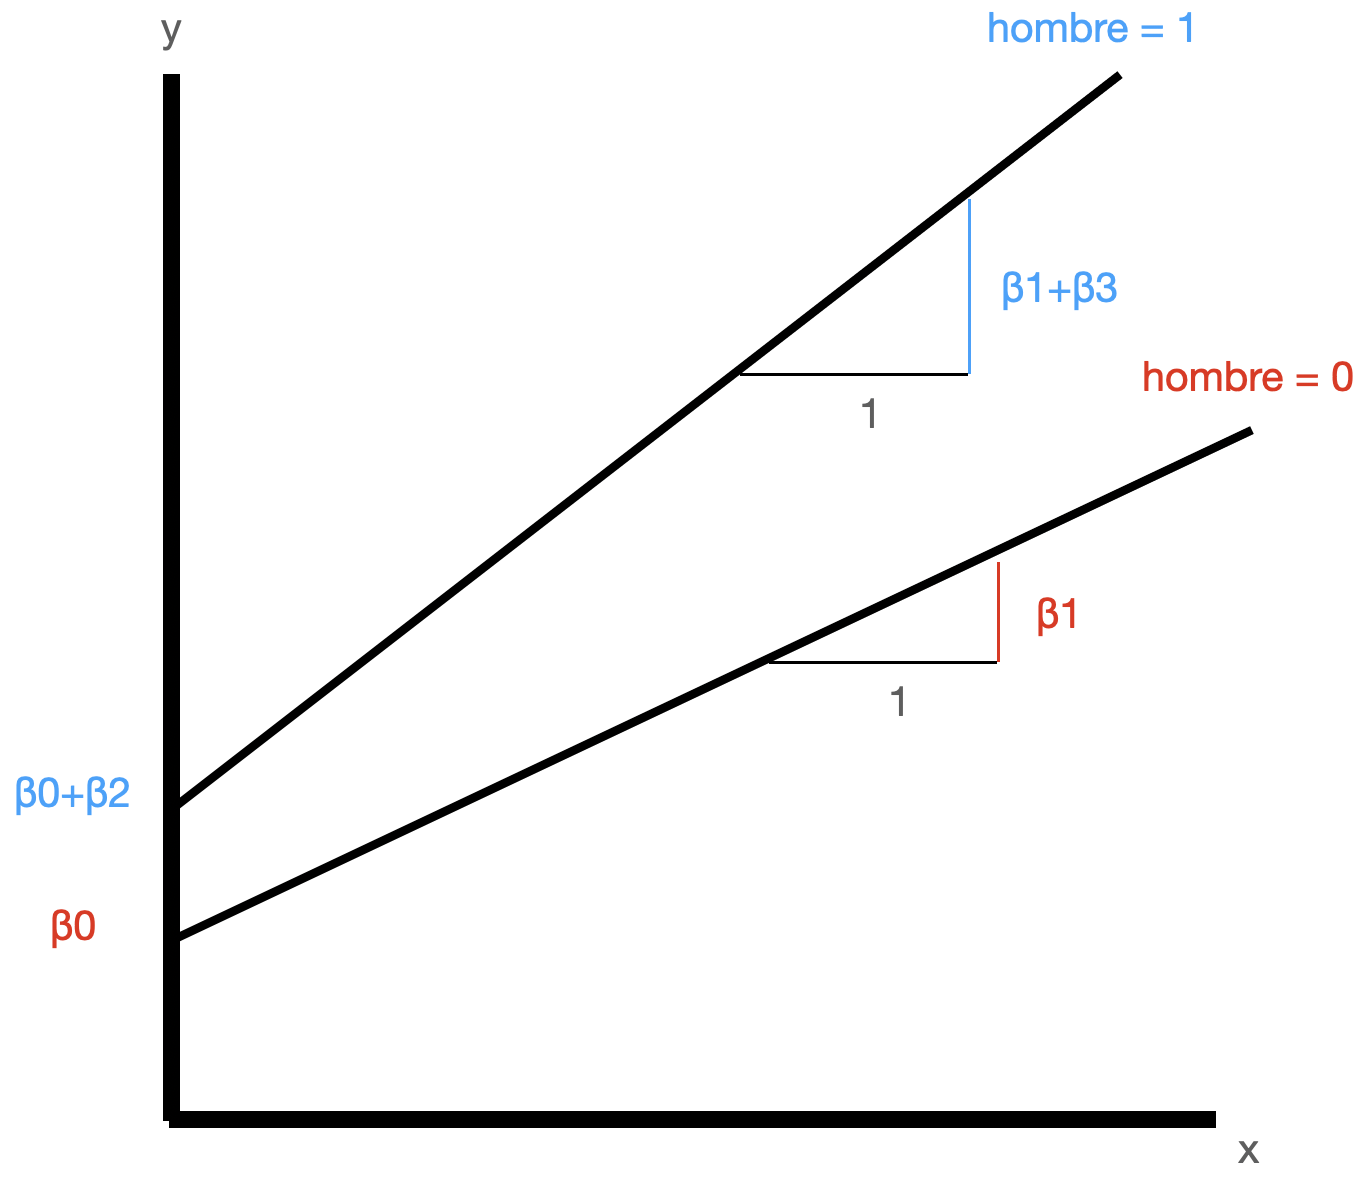
\includegraphics[width=\maxwidth]{it.png}}


%\textcite[71]{Brambor2006} explican que las pendientes $\beta_{1}$ (\autoref{})



\section*{Buenas Pr\'acticas}


F\'ijate que cada vez que incluimos un t\'ermino de interacci\'on ($\text{educaci\'on}_{i} \times {\text{hombre}}_{i}$), para interpretar su par\'ametro asociado ($\beta_{3}$), es necesario incluir los sub-t\'erminos por separado. Esto es, permitir que la ecuaci\'on tenga un par\'ametro independiente asociado a \emph{educaci\'on} y \emph{hombre}, esto es, $\beta_{1}$ y $\beta_{2}$ (tal y como aparece en \autoref{eq:int:term}). Si estimamos s\'olo la siguiente ecuaci\'on, $\beta_{3}$ estar\'a sesgado. {\bf NO HAGAS LO SIGUIENTE}:


    \begin{equation}\label{eq:int:term:mala}
      \text{ingresos}_{i} \;=\; \beta_{0} + \beta_{3}{\text{hombre}}_{i}\times \text{educaci\'on}_{i} + \epsilon_{i}
    \end{equation}



\section*{Estimaci\'on en \texttt{R}}

De acuerdo a \textcite[73]{Brambor2006},\footnote{Ecuaciones 11-13.} el efecto marginal en la ecuaci\'on \autoref{eq:normal},

    \begin{equation}\label{eq:normal}
      \text{ingresos}_{i} \;=\; \beta_{0} + \beta_{1}\text{educaci\'on}_{i} + \beta_{2}\text{hombre}_{i} + \epsilon_{i}
    \end{equation}

est\'a dado por el siguiente c\'alculo:

    \begin{equation}\label{ef:marg:normal}
      \frac{\partial y}{\partial x_{1}} = \beta_{1}
    \end{equation}

Sin embargo el t\'ermino de interacci\'on en \autoref{eq:int:term} es distinto, y est\'a dado por el siguiente c\'alculo:

    \begin{equation}\label{ef:marg:t:i}
      \frac{\partial y}{\partial x_{1}} = \beta_{1} + \beta_{3}\text{hombre}
    \end{equation} % this shows in https://rdrr.io/cran/margins/f/vignettes/Introduction.Rmd Brambor's paper got the equation with a typo. 

En palabras, es \emph{cu\'anto cambia $y$ cuando cambia $x$, seg\'un niveles de la variable hombre}.

Cambiemos de ejemplo, y estimemos un modelo con tres niveles (no dos, como \emph{hombre}).

Carguemos los datos:


\begin{knitrout}
\definecolor{shadecolor}{rgb}{0.969, 0.969, 0.969}\color{fgcolor}\begin{kframe}
\begin{alltt}
\hlkwd{p_load}\hlstd{(effects)}
\hlkwd{data}\hlstd{(Duncan)}
\hlkwd{summary}\hlstd{(Duncan)}
\end{alltt}
\begin{verbatim}
##    type        income        education         prestige    
##  bc  :21   Min.   : 7.00   Min.   :  7.00   Min.   : 3.00  
##  prof:18   1st Qu.:21.00   1st Qu.: 26.00   1st Qu.:16.00  
##  wc  : 6   Median :42.00   Median : 45.00   Median :41.00  
##            Mean   :41.87   Mean   : 52.56   Mean   :47.69  
##            3rd Qu.:64.00   3rd Qu.: 84.00   3rd Qu.:81.00  
##            Max.   :81.00   Max.   :100.00   Max.   :97.00
\end{verbatim}
\end{kframe}
\end{knitrout}

Estimemos el modelo. Nota que hemos puesto la multiplicaci\'on, y \texttt{R} ``sabe'' que debe meter los t\'erminos constitutivos.

\begin{knitrout}
\definecolor{shadecolor}{rgb}{0.969, 0.969, 0.969}\color{fgcolor}\begin{kframe}
\begin{alltt}
\hlstd{modelo.1} \hlkwb{=} \hlkwd{lm}\hlstd{(prestige} \hlopt{~} \hlstd{income}\hlopt{*}\hlstd{type,} \hlkwc{data} \hlstd{= Duncan)}
\hlkwd{summary}\hlstd{(modelo.1)}
\end{alltt}
\begin{verbatim}
## 
## Call:
## lm(formula = prestige ~ income * type, data = Duncan)
## 
## Residuals:
##      Min       1Q   Median       3Q      Max 
## -25.4405  -6.0480  -0.2787   4.7269  28.1950 
## 
## Coefficients:
##                 Estimate Std. Error t value     Pr(>|t|)    
## (Intercept)       2.6828     3.8182   0.703     0.486450    
## income            0.8450     0.1289   6.554 0.0000000882 ***
## typeprof         44.4868    10.3641   4.292     0.000113 ***
## typewc           14.8531    13.4986   1.100     0.277926    
## income:typeprof  -0.2909     0.2017  -1.442     0.157148    
## income:typewc    -0.4674     0.2736  -1.709     0.095466 .  
## ---
## Signif. codes:  0 '***' 0.001 '**' 0.01 '*' 0.05 '.' 0.1 ' ' 1
## 
## Residual standard error: 10.44 on 39 degrees of freedom
## Multiple R-squared:  0.9026,	Adjusted R-squared:  0.8902 
## F-statistic: 72.31 on 5 and 39 DF,  p-value: < 0.00000000000000022
\end{verbatim}
\end{kframe}
\end{knitrout}

Como explican \textcite{Brambor2006}, las tablas de regresi\'on no nos ayudan a interpretar los modelos interactivos. Debemos proceder interpretando como se se\~nala en \autoref{ef:marg:t:i}. Afortunadamente existe la librer\'ia \texttt{effects}.


\begin{knitrout}
\definecolor{shadecolor}{rgb}{0.969, 0.969, 0.969}\color{fgcolor}\begin{kframe}
\begin{alltt}
\hlstd{term.int} \hlkwb{<-} \hlkwd{effect}\hlstd{(}\hlstr{"income*type"}\hlstd{, modelo.1)}
\hlkwd{plot}\hlstd{(term.int,} \hlkwc{as.table}\hlstd{=T)}
\end{alltt}
\end{kframe}

{\centering 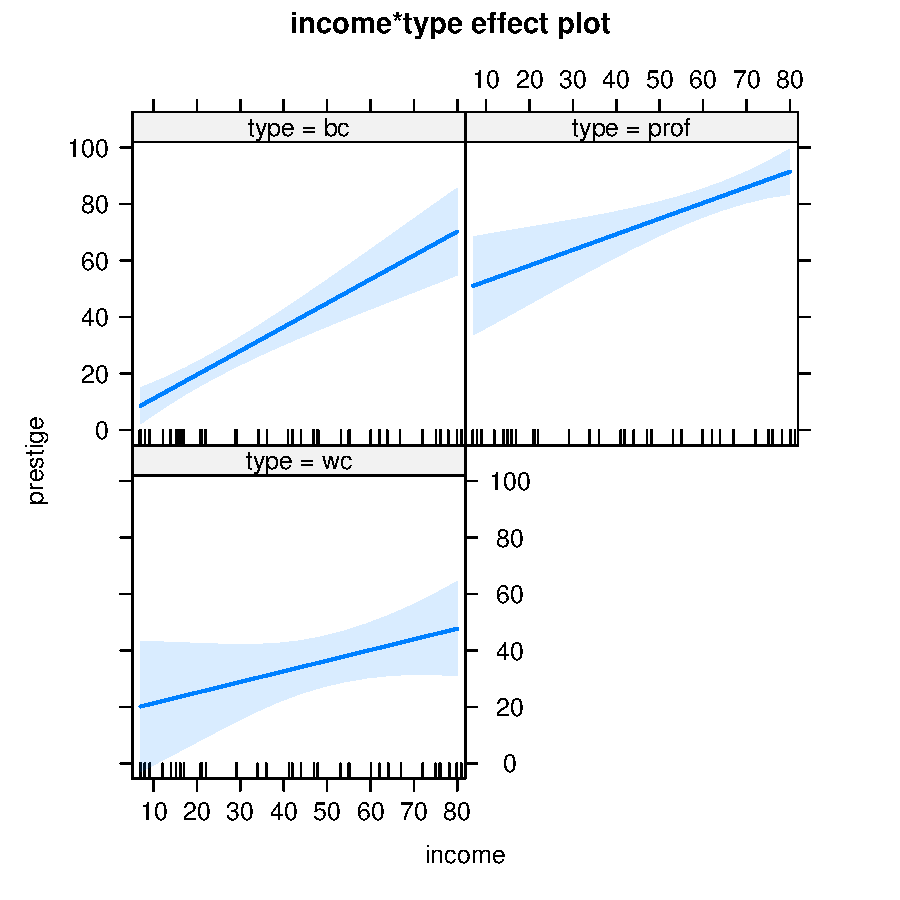
\includegraphics[width=\maxwidth]{figure/i:c:3-1} 

}



\end{knitrout}


Si te das cuenta, los efectos no son los mismos. Las derivadas (en \autoref{ef:marg:t:i}) no tienen por qu\'e dar lo mismo. Es por esto que no debemos mirar la tabla de regresi\'on. En un sentido espacial, un t\'ermino de interacci\'on es el an\'alisis de tres planos. En la \autoref{eq:int:term}: $y$, $x_{1}$, $x_{2}$. 

Veamos de qu\'e se trata:

\begin{knitrout}
\definecolor{shadecolor}{rgb}{0.969, 0.969, 0.969}\color{fgcolor}\begin{kframe}
\begin{alltt}
\hlkwd{p_load}\hlstd{(scatterplot3d)}
\hlkwd{scatterplot3d}\hlstd{(Duncan}\hlopt{$}\hlstd{income, Duncan}\hlopt{$}\hlstd{type, Duncan}\hlopt{$}\hlstd{prestige,} \hlkwc{color} \hlstd{=} \hlkwd{as.numeric}\hlstd{(Duncan}\hlopt{$}\hlstd{type))}
\end{alltt}
\end{kframe}

{\centering 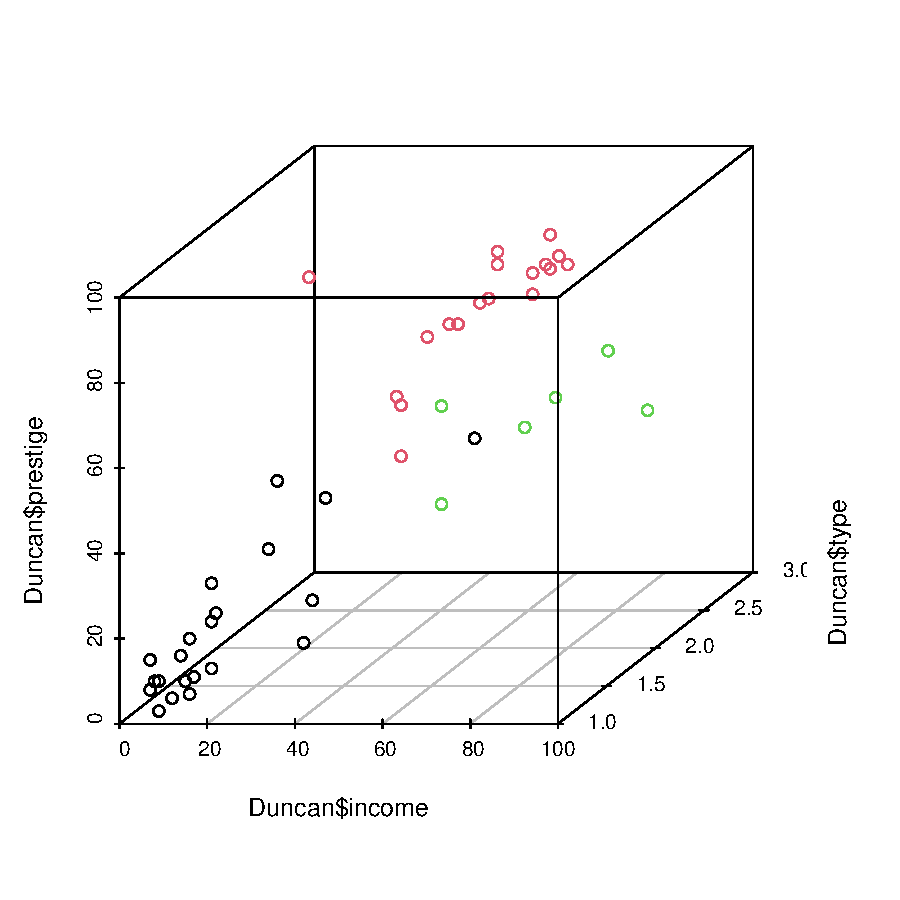
\includegraphics[width=\maxwidth]{figure/i:c:4-1} 

}



\end{knitrout}

Usemos una base de datos donde todas las variables son continuas (no como en el ejemplo donde \emph{hombre} es dicot\'omica):

\begin{knitrout}
\definecolor{shadecolor}{rgb}{0.969, 0.969, 0.969}\color{fgcolor}\begin{kframe}
\begin{alltt}
\hlkwd{p_load}\hlstd{(car,rgl)}
\hlkwd{data}\hlstd{(iris)}
\hlstd{sep.l} \hlkwb{<-} \hlstd{iris}\hlopt{$}\hlstd{Sepal.Length}
\hlstd{sep.w} \hlkwb{<-} \hlstd{iris}\hlopt{$}\hlstd{Sepal.Width}
\hlstd{pet.l} \hlkwb{<-} \hlstd{iris}\hlopt{$}\hlstd{Petal.Length}
\hlkwd{scatter3d}\hlstd{(}\hlkwc{x} \hlstd{= sep.l,} \hlkwc{y} \hlstd{= pet.l,} \hlkwc{z} \hlstd{= sep.w,} \hlkwc{groups} \hlstd{= iris}\hlopt{$}\hlstd{Species)}
\end{alltt}
\end{kframe}
\end{knitrout}

Correr esto \'ultimo en \texttt{R}.

\begin{knitrout}
\definecolor{shadecolor}{rgb}{0.969, 0.969, 0.969}\color{fgcolor}\begin{kframe}
\begin{verbatim}
## [1] "Clase_14.R"
## Writing to file Clase_14.R
\end{verbatim}
\end{kframe}
\end{knitrout}
%\newpage
%\paragraph{}
%\paragraph{}
%\pagenumbering{Roman}
%\setcounter{page}{1}
%\printbibliography

\end{document}


